
\begin{figure*}[!t]
    \centering{}
	\subfloat[IOPS] { 
	    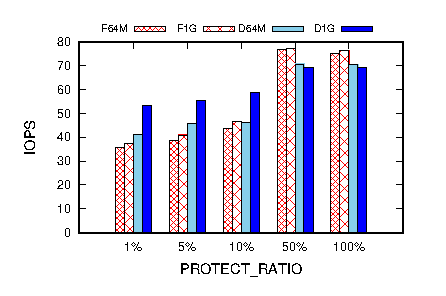
\includegraphics[width=0.3\textwidth]{expr/micro_rslt_220525/perf/perf_RAND.eps}
	    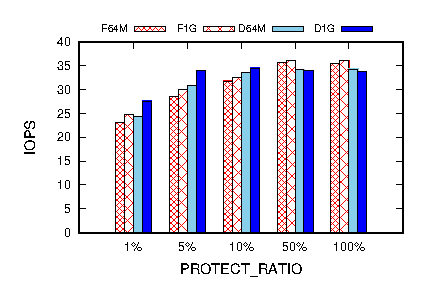
\includegraphics[width=0.3\textwidth]{expr/micro_rslt_220525/perf/perf_JESD.eps}
	    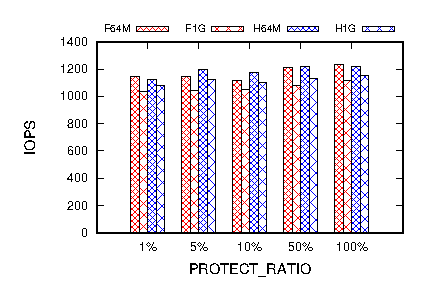
\includegraphics[width=0.3\textwidth]{expr/macro_rslt_220601/perf/perf_OLTP.eps}
	} \\
<<<<<<< HEAD
	\subfloat[WAF (UD: User Data, MD: Mapping Data, GUD/GMD: GC for User/Mapping Data)] { 
=======
	\subfloat[Write Traffic (UD: User Data, MD: Mapping Data, GUD/GMD: GC for User/Mapping Data)] { 
>>>>>>> 3265b4e384efcf72fe616b15a5b7b0dc6d1ce99d
	    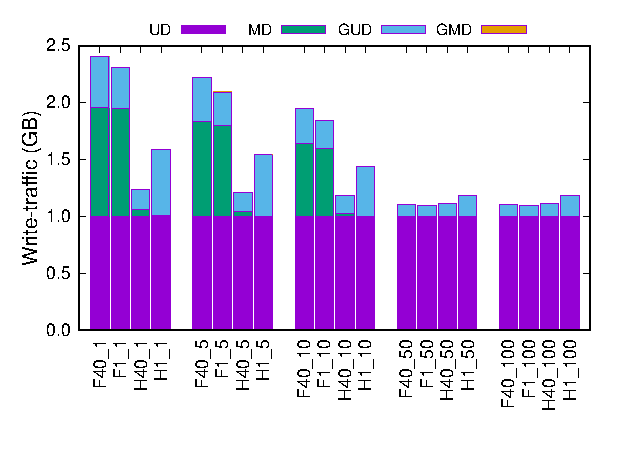
\includegraphics[width=0.3\textwidth]{expr/micro_rslt_220601/waf/RAND_waf.eps}
        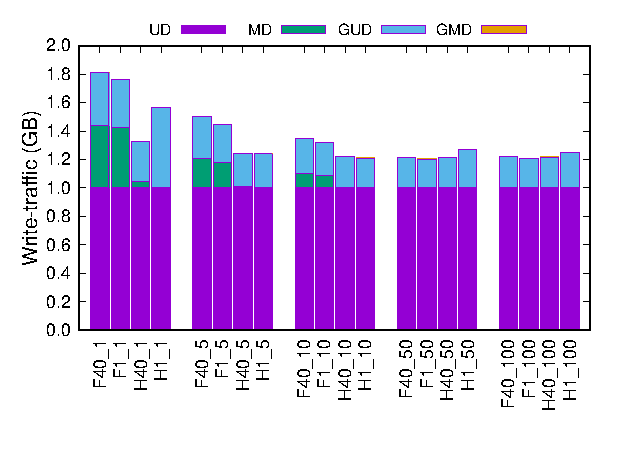
\includegraphics[width=0.3\textwidth]{expr/micro_rslt_220601/waf/JESD_waf.eps}
        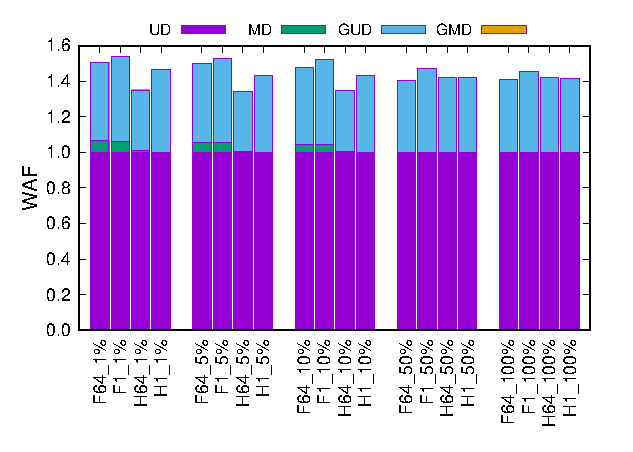
\includegraphics[width=0.3\textwidth]{expr/macro_rslt_220601/waf/OLTP.eps}
	} 
    % \caption{\textbf{IOPS}:\textit{F and H denotes FIFO and HEXA.}}
<<<<<<< HEAD
    \caption{\textbf{IOPS and WAF.} From left: Random, JESD, and TPC-C.}
=======
    \caption{\textbf{IOPS and Write Traffic.} From left: Random, JESD, and TPC-C.}
>>>>>>> 3265b4e384efcf72fe616b15a5b7b0dc6d1ce99d
    \label{fig_perf_iops}
    \vspace{-15pt}
\end{figure*} 

\iffalse
\begin{figure*}[!t]
    \centering{}
	\subfloat[IOPS] { 
	    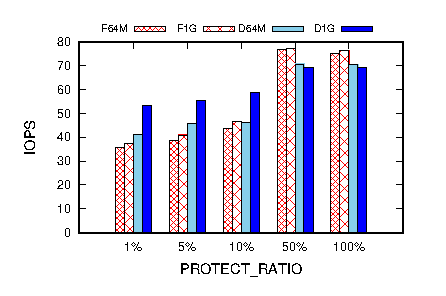
\includegraphics[width=0.3\textwidth]{expr/micro_rslt_220525/perf/perf_RAND.eps}
	    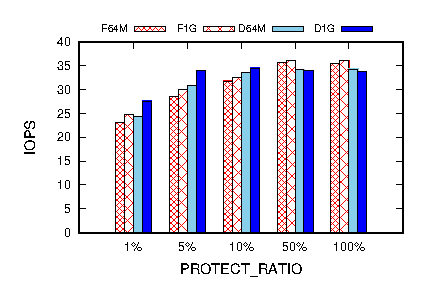
\includegraphics[width=0.3\textwidth]{expr/micro_rslt_220525/perf/perf_JESD.eps}
	    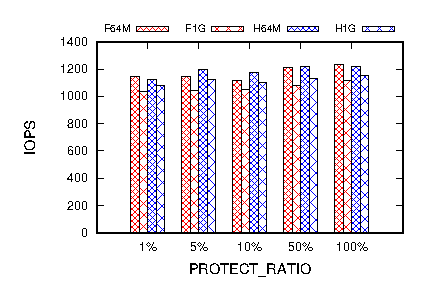
\includegraphics[width=0.3\textwidth]{expr/macro_rslt_220601/perf/perf_OLTP.eps}
	} \\
	\subfloat[Write Traffic] { 
	    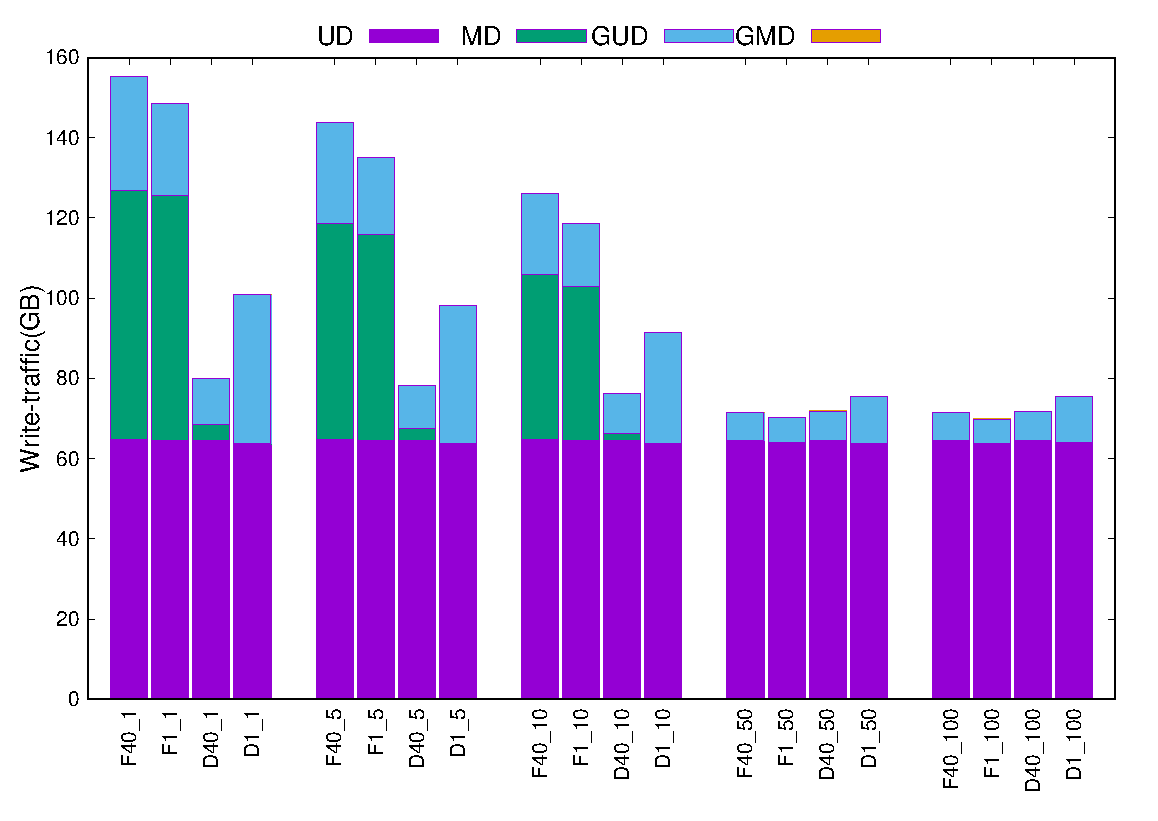
\includegraphics[width=0.3\textwidth]{expr/micro_rslt_220525/wt/RAND.eps}
        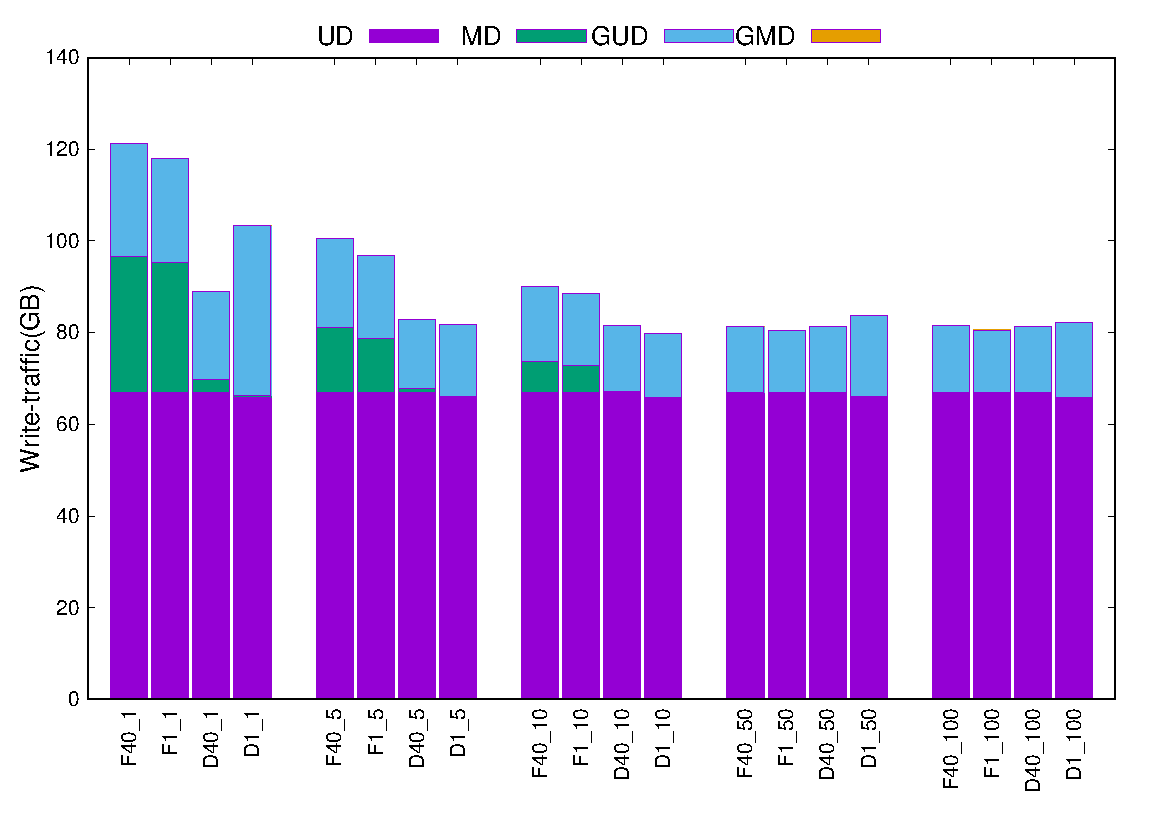
\includegraphics[width=0.3\textwidth]{expr/micro_rslt_220525/wt/JESD.eps}
        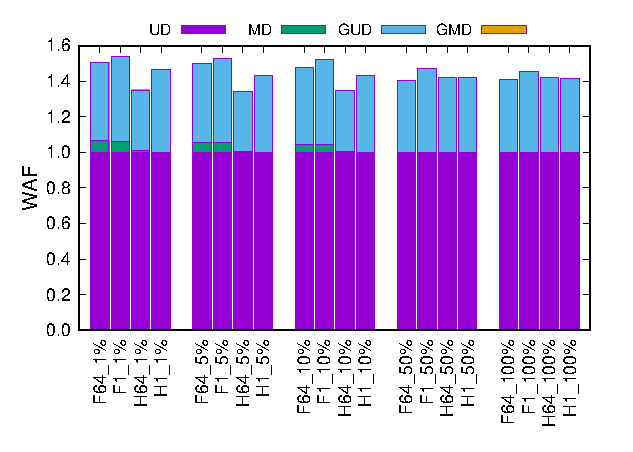
\includegraphics[width=0.3\textwidth]{expr/macro_rslt_220601/waf/OLTP.eps}
	} 
    % \caption{\textbf{IOPS}:\textit{F and H denotes FIFO and HEXA.}}
    \caption{\textbf{IOPS and Write Traffic.}}
    \label{fig_perf_iops}
    \vspace{-15pt}
\end{figure*} 
\fi
\iffalse
\begin{figure*}[!t]
    \centering{}
	\subfloat[Random] { 
	    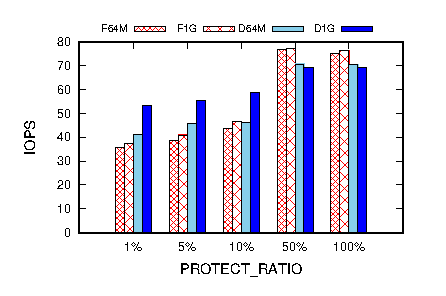
\includegraphics[width=0.3\textwidth]{expr/micro_rslt_220525/perf/perf_RAND.eps}
	} 
	\subfloat[JESD] { 
	    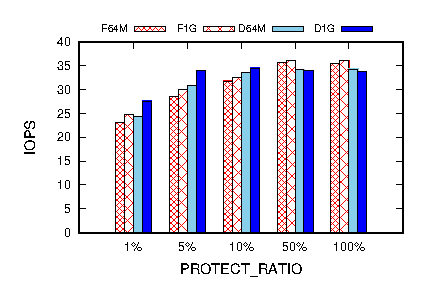
\includegraphics[width=0.3\textwidth]{expr/micro_rslt_220525/perf/perf_JESD.eps}
	}
	\subfloat[TPC-C] {
	    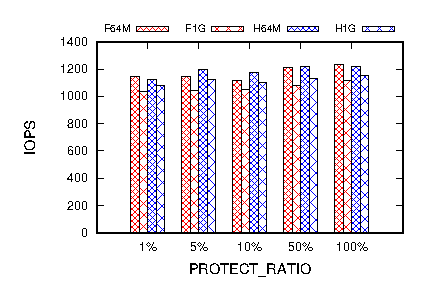
\includegraphics[width=0.3\textwidth]{expr/macro_rslt_220601/perf/perf_OLTP.eps}
	} \\
%     \subfloat[TPC-C] {
% 	    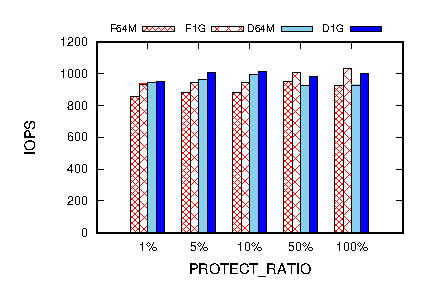
\includegraphics[width=0.3\textwidth]{expr/macro_rslt_220525/perf/perf_OLTP.eps}
% 	}
	\subfloat[Random] { 
	    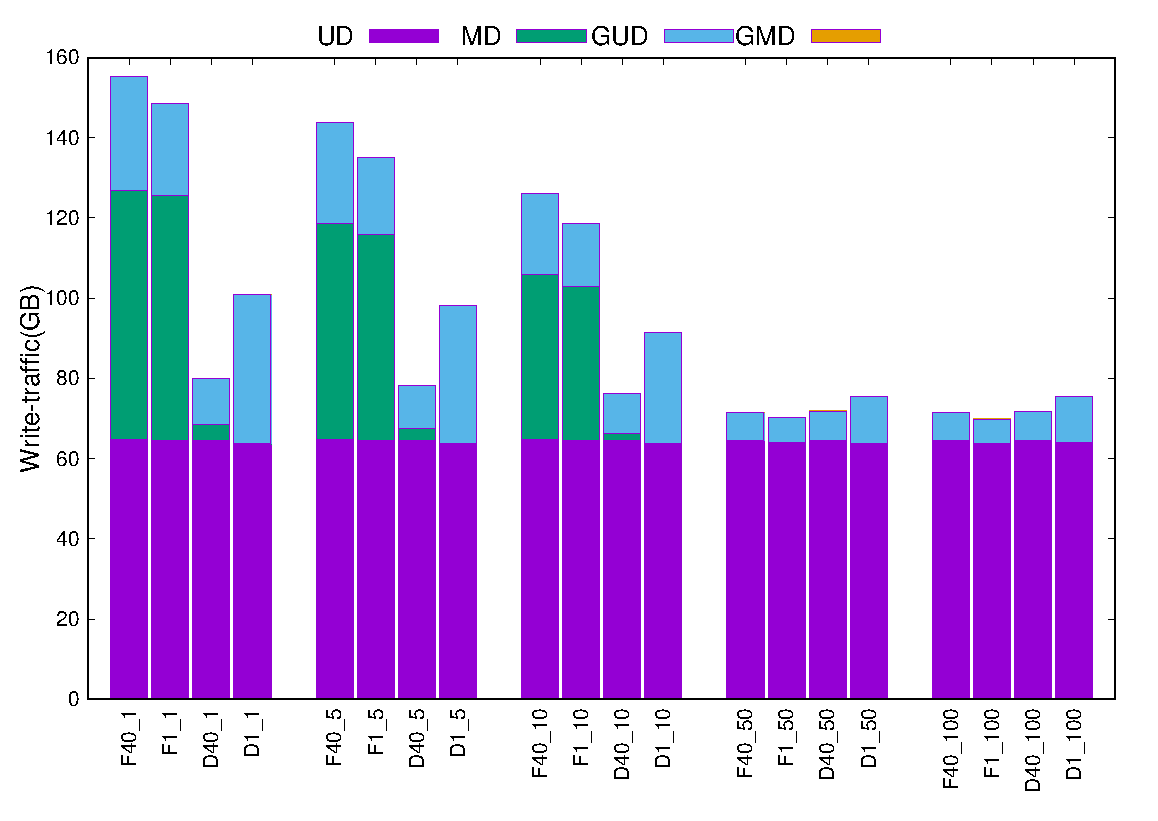
\includegraphics[width=0.3\textwidth]{expr/micro_rslt_220525/wt/RAND.eps}
	} 
	\subfloat[JESD] { 
	    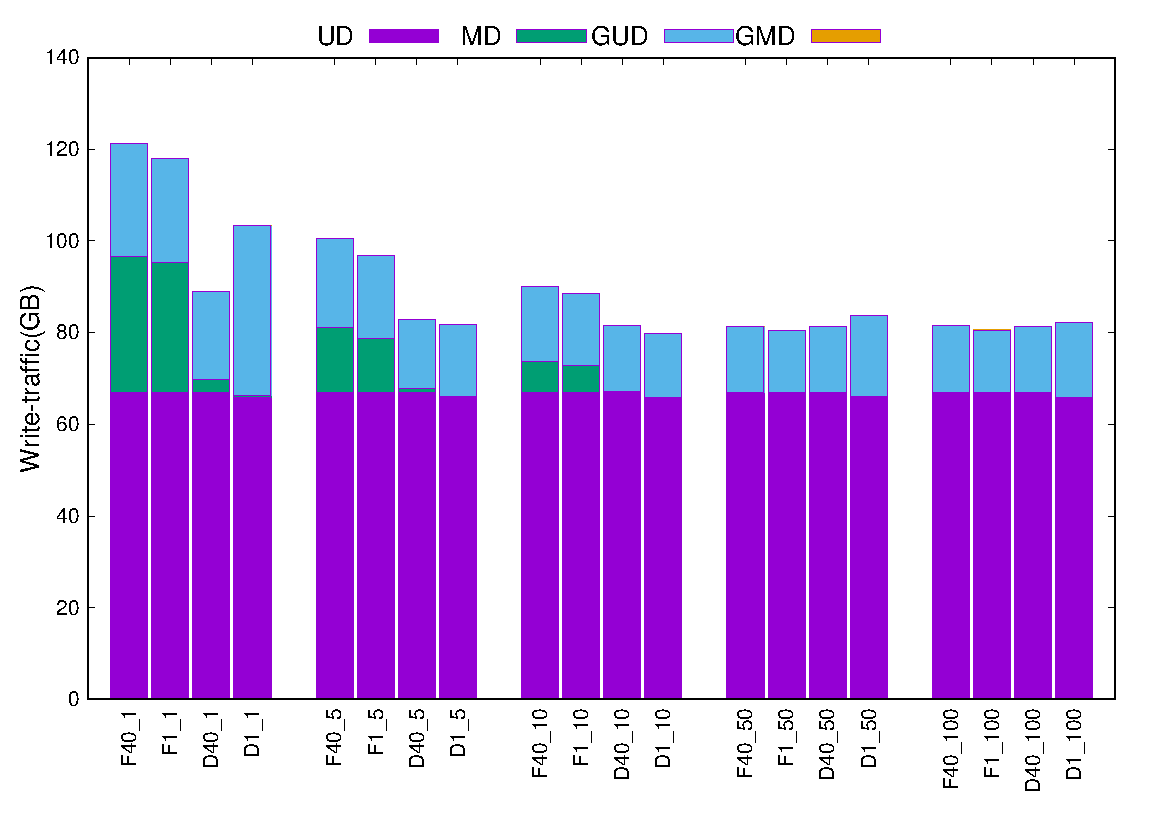
\includegraphics[width=0.3\textwidth]{expr/micro_rslt_220525/wt/JESD.eps}
	}
% 	\subfloat[TPC-C] { 
% 	    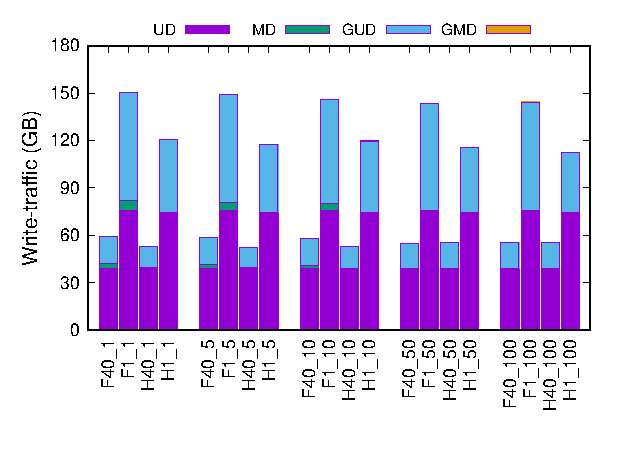
\includegraphics[width=0.3\textwidth]{expr/macro_rslt_220525/wt/OLTP.eps}
% 	}
	\subfloat[TPC-C] { 
	    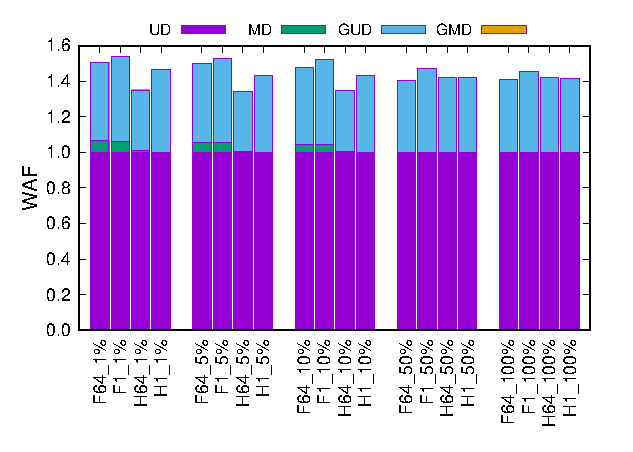
\includegraphics[width=0.3\textwidth]{expr/macro_rslt_220601/waf/OLTP.eps}
	}
    % \caption{\textbf{IOPS}:\textit{F and H denotes FIFO and HEXA.}}
    \caption{\textbf{IOPS and Write Traffic.}}
    \label{fig_perf_iops}
    \vspace{-15pt}
\end{figure*} 
\fi

\iffalse
\begin{figure*}[!t]
    \centering{}
	\subfloat[Random] { 
	    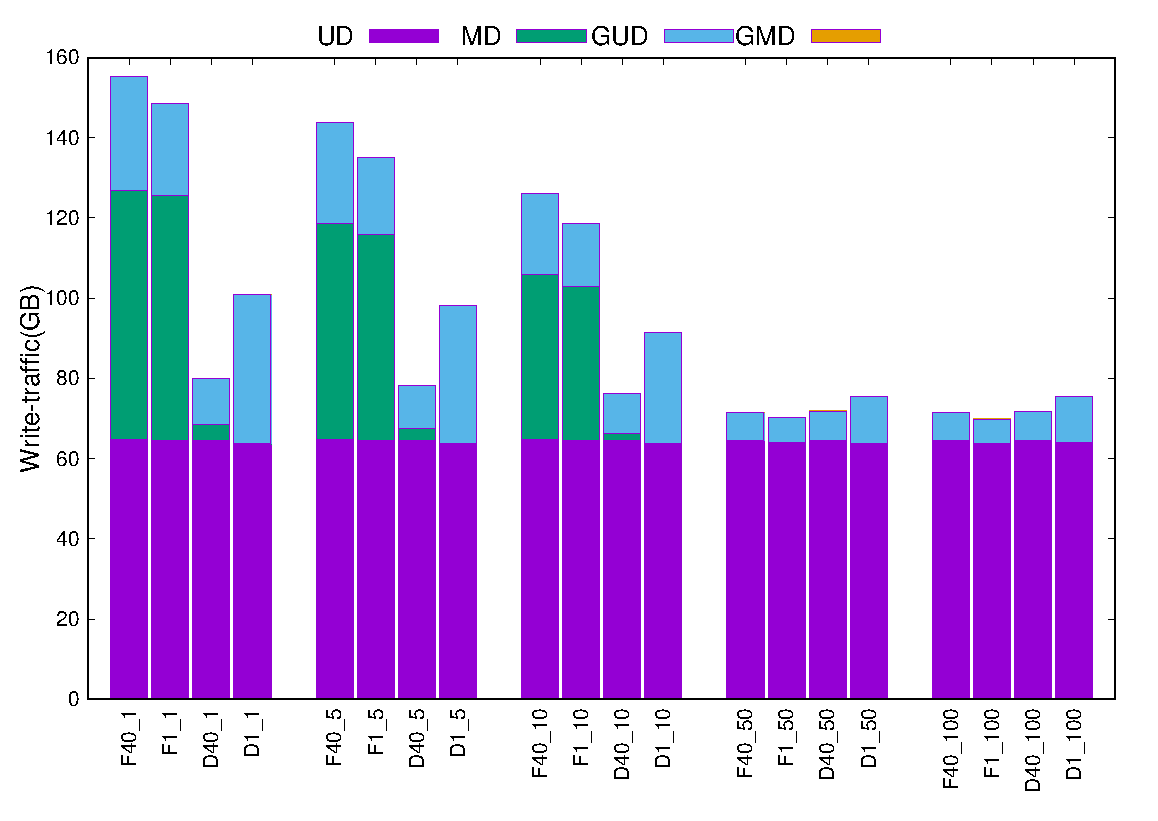
\includegraphics[width=0.3\textwidth]{expr/micro_rslt_220525/wt/RAND.eps}
	} 
	\subfloat[JESD] { 
	    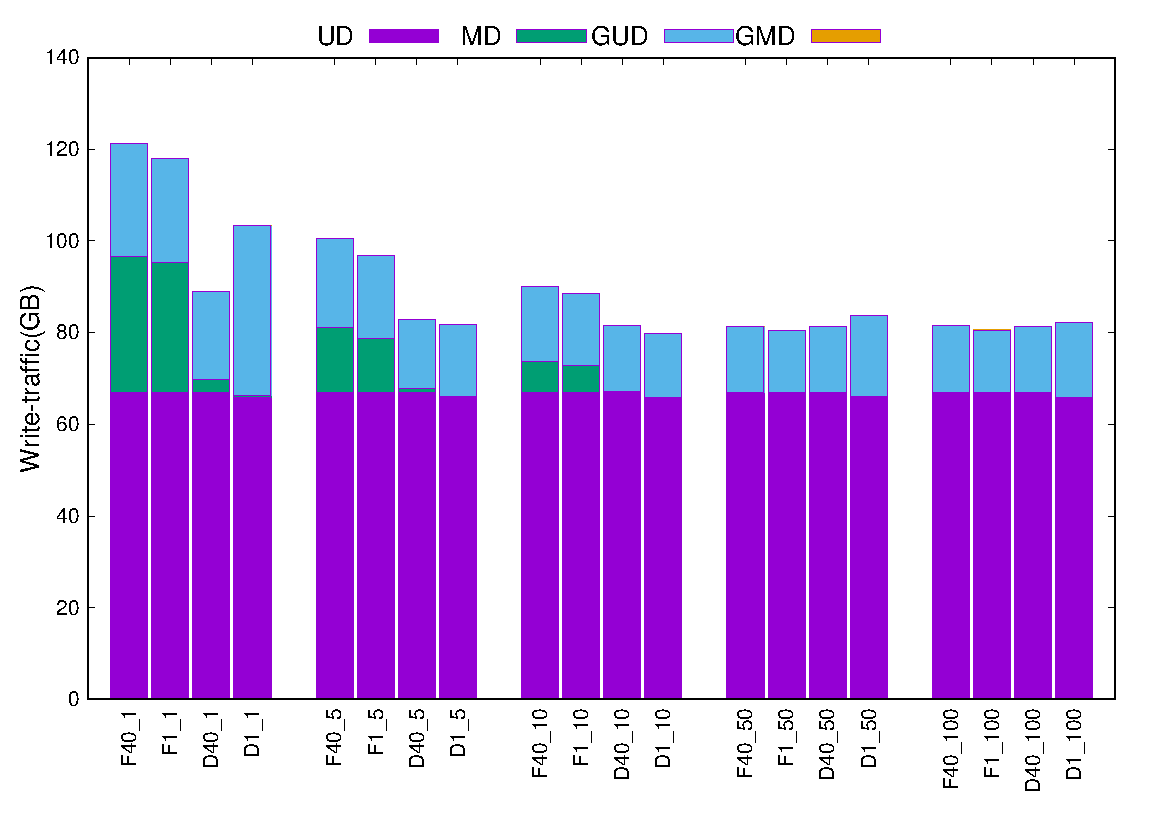
\includegraphics[width=0.3\textwidth]{expr/micro_rslt_220525/wt/JESD.eps}
	}
% 	\subfloat[TPC-C] { 
% 	    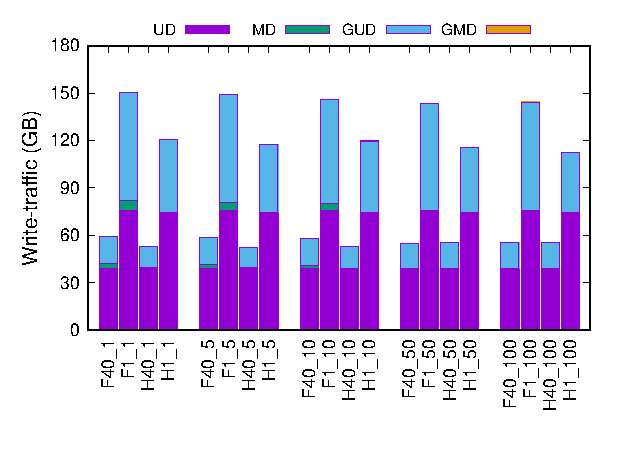
\includegraphics[width=0.3\textwidth]{expr/macro_rslt_220525/wt/OLTP.eps}
% 	}
	\subfloat[TPC-C] { 
	    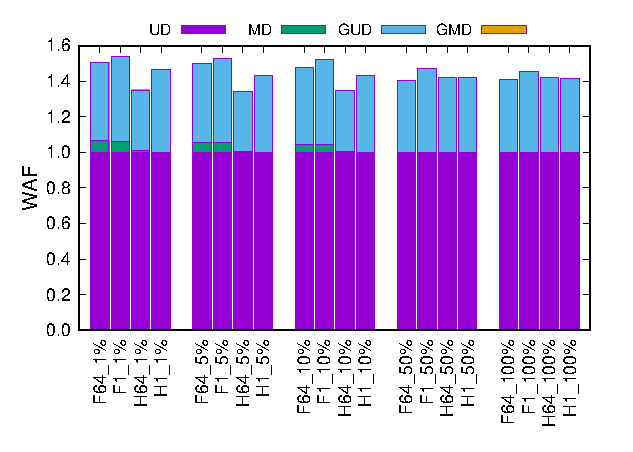
\includegraphics[width=0.3\textwidth]{expr/macro_rslt_220601/waf/OLTP.eps}
	}
	\caption{\textbf{Write Traffic.} \textit{UD - User Data, MD - Mapping Data, GUD - GC Write for User Data, GMD - GC Write for Mapping Data.}}
    \label{fig_perf_wt}
\end{figure*} 
\fi



\section{Evaluation}
%We assume 1\% of the mapping table is protected via capacitors in a 64GB SSD. 
%The 64GB SSD is using DRAM and assumes that 1\% of the mapping table is
%protected. 
We perform the experiments on a machine with a 20-core Intel Xeon(R) Silver
4114 CPU running at 2.2GHz and 84GB memory. We run FEMU (QEMU-based SSD
emulator) configured to use 10 cores, 4GB DRAM for main memory, and 16GB DRAM
for SSD emulation. We use a page-level mapping and caches all translation pages in DRAM. 
The NAND flash chips include 8 channels and 8 flash
LUNs per channel. The page size is 8KB and the per-block pages are 256. The
read and write latency is set to 60us and 700us,
respectively~\cite{cheong2018flash}. We use the greedy algorithm for
GC(Garbage-Collection) and mount an Ext4 file system on the device.
% , which selects the least utilized block as a victim for cleaning. 
% The Ext4 file system is mounted on the emulated SSD.  
%Other configuration uses default settings of FEMU 

% We measure the average IOPS and the write traffic varying the protected ratio of a mapping table from 1\% to 100\%. 
The performance evaluation is conducted using three workloads.
% The fio benchmark~\cite{fio-bench} generates the 4KB of random writes and the
The fio benchmark generates the 4KB of random writes and the
skewed read-write mixed workload that follows JESD219 using 4 threads. A
total of 64GB of data was written to the 4GB area. For the real workload, we use 
TPC-C~\cite{council1990tpc} on MySQL, an online transactional processing benchmark.
% , which is executed using a sysbench benchmark suite~\cite{sysbench}.
For TPC-C, we precondition an SSD so that the 75\% of capacity is filled with data
and perform 0.1 million of write queries using 10 threads.
% The TPC-C preconditions an SSD with data writes for 300 seconds and generates  
% write quries for 180 seconds using 10 threads.
For the performance comparison, we also implemented an FIFO-SSD that processes 
write requests in arrival order.  

Fig.\ref{fig_perf_iops} shows the IOPS and WAF (Write Amplification Factor) of FIFO-SSD and \ours{} (denoted with a prefix F and H) when varying the protected ratio of a mapping table from 1\% to 100\%. 
We study two different sizes of write
buffer, 64MB and 1GB, to investigate the effectiveness of \ours{} with respect
to the queue depth. 
\iffalse
랜덤 워크로드에서 Hexa-SSD의 성능 향상폭이 가장 큼. mapping table locality 가 낮아 protected ratio 가 낮으면 mapping table flush 로 인한 traffic 증가가 컸음. 
\ours{}는 buffer 내의 request re-ordering 을 통해 mapping table flush overhead 를 거의 제거함. 
이에 protected ratio 가 1\% 이고 WB가 1GB일 때, WAF를 기존 2.3 인 것을 1.5로 낮춤. 
이에 따른 성능향상도 1.4x 가 됨. 
\fi
As the figure shows, the random workload improves the most with \ours{}. 
This workload natively has low spatial locality, and thus it benefits enormously from the re-ordering of \ours{}. In particular, the performance greatly improves when the buffer size is large. 
Consequently, \ours{} with 1GB buffer lowers WAF from 2.3 to 1.5 and enhances IOPS by 42.7\% when the protection ratio is 1\%. 
\iffalse
JESD에서도 전체적인 트렌드는 비슷하나 write traffic 의 감소폭과 성능향상폭은 다소 줄어들었다. 
그 이유는 JESD워크로드가 원래random 보다 mapping table update 에 locality 가 있기 때문임. 
이에 protected ratio 가 1\% 일때 WAF는 1.8과 1.7이던 것이 1.3과 1.5로 감소함. 
성능은 최대 13\% 향상됨. 
\fi
For JESD, the result shows the same general trends as for the random workload, while the performance gain
becomes smaller as it has more skewed access patterns. 

TPC-C exhibits the disparate outcome. Although it reduces write amplification by up to 7\% in \ours, the performance has no remarkable improvement with it. 
Furthermore, IOPS buffer size is small. 

\iffalse
TPC-C는 WAF는 최대 7\% 까지 감소시켰으나 성능은 \ours{}와 FIFO-SSD가 거의 비슷하게 관찰됨. 
그 이유는 TPC-C 자체도 지역성이 높아 re-ordering 으로 인한 write traffic 감소폭도 작고, FIO benchmark (얘는 direct 로 실행)와 달리 상위 소프트웨어 스택이 높아서 백그라운드로 동작하는 ssd 내부의 write traffic 변화가 민감하게 user-perceived performance 에 영향을 끼치지 않는 것으로 파악되었다. 
한편, 다른 워크로드와는 달리 버퍼가 작을 때 성능이 더 좋았다. 정확한 이유는 모르겠으나, 버퍼 크기가 커짐에 따라 FTL 내의 자료구조가 복잡해져 소프트웨어 오버헤드가 성능에 영향을 끼친 것으로 추측된다. 
\fi

\iffalse
When the protected ratio is less than 10\%, \ours{} has improved the performance by up to XX\% compared to the existing FIFO version.
Compared with full protection SSD, when the protected ratio is 1\%, FIFO performance degradation occurs more than XX\%-XX\%, whereas in \ours{}, performance degradation is XX\% - XX\%. This performance enhancement is achieved by significantly reducing the cost of flushing overflew dirty pages to the SSD through the in-buffer re-ordering.
\fi
\iffalse
protected ratio 가 10\% 이하일 때 DAWID 이 기존 FIFO 방식 버전보다 최대 XX\%
성능을 향상시켰다.  Full protected 경우와 비교하면 protected ratio 가 1\%로
줄어들 때 FIFO는 성능저하가 XX\%-XX\% 이상 발생하는 반면, DAWID은 성능저하가
XX\% - XX\% 에 머물렀다.  이러한 성능향상 효과는 mapping table 의 영속성을 위해
dirty page 를 SSD에 flush 하는 오버헤드를 in-buffer re-ordering 을 통해 상당히
많이 줄였기 때문이다. 
Fig.~\ref{fio_perf_wt}에서 보는바와 같이 DAWID은 protected ratio 가 작을 때에도
mapping table flush 오버헤드를 거의 없애 FIFO 대비 쓰기량을 최대 XX\%까지 절감하였다. 
\fi

\iffalse
한가지 예상치 못한 결과는 protected ratio 가 50\% 이상일 때 DAWID이 FIFO보다
IOPS가 살짝 낮다는 것이다. In-depth analysis 를 수행한 결과 reordering 이 host
에서 발생시키는 본연의 write pattern 을 distort 하게 되는데 이로 인해 lifetime
이 다른 page 들이 동일 블록에 저장되는 가능성을 높이기 때문이다. 결과적으로
이는 GC에서 copy 해야 하는 valid page 의 숫자를 증가시켜 GC의 write traffic 을
늘린다.  워크로드가 synthetic random 인 상황에서도 파일시스템을 거쳐서 들어오기
때문에 temporal locality 를 가짐. 이에 re-ordering 을 통한 host write pattern
의 왜곡이 GC의 성능 저하를 일으키게 됨. 본 논문에서 targeting 하는 상황은
protected ratio 가 낮은 경우이지만 기법의 적용성(?)을 향상시키기 위해 상기 문제를 
완화시킬 수 있는 기법에 대해 향후 연구해보고자 합. 
\fi

One counter-intuitive result is that \ours{} has slightly lower IOPS than FIFO when protected ratio is above 50\%. Our careful analysis reveals that the reordering of \ours{} distorts the original write pattern generated by the host, which increases the possibility that pages with different lifetimes are stored in the same block. As a result, this increases the number of valid pages that need to be copied from the GC, thereby increasing the write traffic of the GC. Even when the workload is synthetic random, the host writes have temporal locality because they are transferred through a file system. 
%Therefore, distortion of host write pattern through re-ordering causes degradation of GC performance. 
Nevertheless, note that the target environment of this paper is a case where the protected ratio is low, but in order to improve the generality of \ours{}, we will study the technique that can alleviate the above problem in the future.


%\begin{figure*}[t]
%    \centering{}
%	\subfloat[OLTP] { 
%	    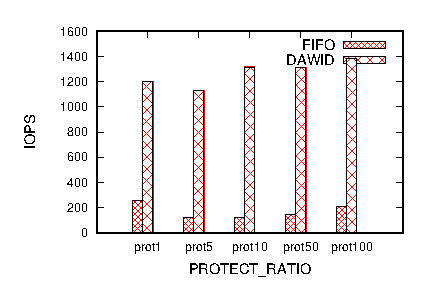
\includegraphics[width=0.3\textwidth]{expr/macro_220517/perf/OLTP/perf_OLTP.eps}
%	} 
%	\subfloat[Write Traffic] { 
%	    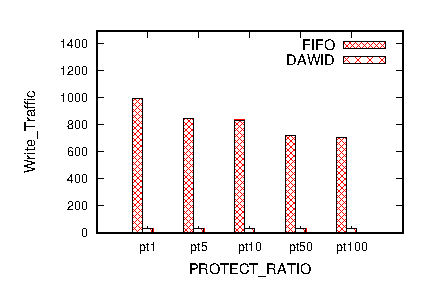
\includegraphics[width=0.3\textwidth]{expr/macro_220517/wt/OLTP/perf_OLTP.eps}
%	} 
%    \caption{\textbf{OLTP}}
%\end{figure*} 



%\begin{figure*}[t]
%    \centering{}
%	\subfloat[Sequential] { 
%	    %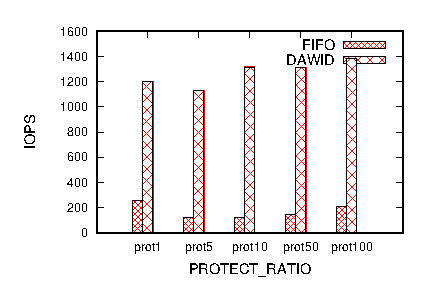
\includegraphics[width=0.3\textwidth]{expr/macro_220517/perf/OLTP/perf_OLTP.eps}
%	    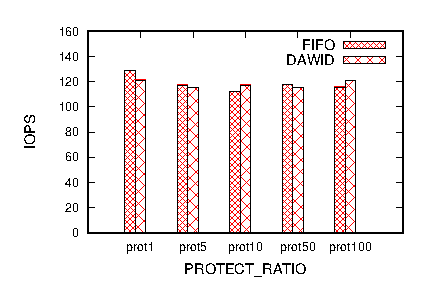
\includegraphics[width=0.3\textwidth]{expr/micro_220517/perf/SEQ/perf_SEQ.eps}
%	} 
%	\subfloat[Random] { 
%	    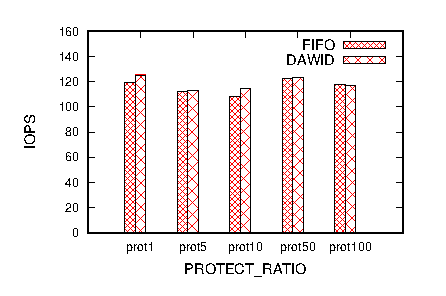
\includegraphics[width=0.3\textwidth]{expr/micro_220517/perf/RAND/perf_RAND.eps}
%	} 
%	\subfloat[JESD] { 
%	    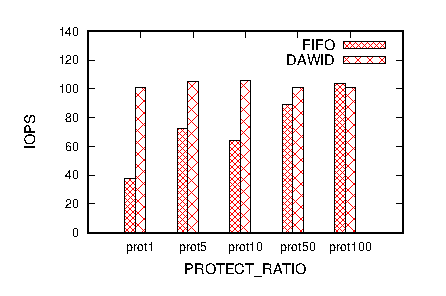
\includegraphics[width=0.3\textwidth]{expr/micro_220517/perf/JESD/perf_JESD.eps}
%	}
%    \caption{\textbf{IOPS}}
%\end{figure*} 
%



